
%Diese LaTeX-Vorlage f�r Praktikumsprotokolle in Form einer Ver�ffentlichung f�r das 
%F-Praktikum wurde erstellt von Andreas Nuber EP II, Uni W�rzburg.
%Es wurde das Koma-Skript verwendet und sollte somit installiert sein
%desweiteren sollten alle packages installiert sein, die mit \usepackage{} 
%eingebunden werden.
%Zum Testen dieser Vorlage wurde MikTex verwendet sowie TeXnicCenter als Editor
%beim Compilieren waren 0 Fehler, 1 Warnung und 3 zu volle/leere Boxen. Das ist ok :)

%F�r das Erstellen einfach den sinnfreien Text, der zum ausf�llen genommen wurde 
%ersetzen. Was sonst noch ver�ndert werden sollte steht in den Kommentaren!


\documentclass[a4paper,10pt,twocolumn]{scrartcl} %Koma-Skript-�quivalent zu "article"

\usepackage{german}            %macht deutsche �berschriften
\usepackage[latin1]{inputenc}  %man kann Sonderzeiche wie �,� usw direkt eingeben
\usepackage{amsmath}           %macht
\usepackage{amsfonts}          %Mathe
\usepackage{amssymb}           %m�chtiger
\usepackage{graphicx}          %erlaubt Graphiken einzubinden (.eps f�r dvi und ps sowie .jpg f�r pdf)
\usepackage[T1]{fontenc}       %Zeichenbelegung der verwendeten Schrift
\usepackage{ae}                %macht sch�neres �
\usepackage{typearea}	       %erm�glicht �nderung des Seitenspiegels
\usepackage{scrlayer-scrpage}  %erm�glicht �nderung der Kopf-/Fu�zeile
\usepackage{lastpage}          %l�sst auf die Seienanzahl zugreifen
\usepackage[margin=10pt,font=small,labelfont=bf]{caption} %macht die Bildbeschriftungen richtig
\usepackage{siunitx}
\usepackage{url}
\usepackage{placeins}
\usepackage[nodayofweek]{datetime} 
\usepackage{textgreek}

%\renewcommand{\figurename}{Abb.}

\pagestyle{scrheadings}        %sagt Koma-Skript, dass selbstdefiniers Kopfzeilen verwendet werden
\typearea{16}                  %stellt Seitenspiegel ein
\columnsep25pt				   %definiert Breite zwischen den zwei Spalten von \twocolumns

\renewcommand{\pnumfont}{%     %�ndert die Schriftart der Seitennummerierung
\normalfont\rmfamily\slshape}  %�ndert die Schriftart der Seitennummerierung 
\renewcommand\refname{References}
\renewcommand{\figurename}{Fig.}
\renewcommand{\tablename}{Tab.}

\begin{document}
\cfoot{\thepage /\pageref{LastPage}}     %macht die Seitennumerierung der Fom 2/5 (ausser auf der Titelseite)

\twocolumn[{\csname @twocolumnfalse\endcsname                %erlaubt "Abstrakt" �ber beide Spalten
\titlehead{                                                  %Kopfzeile
	\begin{tabular*}{\textwidth}[]{@{\extracolsep{\fill}}lr}   %Kopfzeile
	Instructor: Tobias Kie�ling & \today\\                          %Kopfzeile      hier den Betreuer eintragen!!!
	\end{tabular*}                                             %Kopfzeile
	}
\title{Measuring propagation speeds of ultrasound in different media and non-destructive material analysis with ultrasound}	    %Titel der Versuchs
\author{Jonas Beck and Jonathan Bodky		}                   %Namen der Studenten
\date{}                                                         %ben�tigt um automatisches Datum auszuschalten
\maketitle                                                      %erzeugt Titelseite
\vspace{-8ex}                                                   %verringert Abstand zur �berschrift
\begin{abstract}                                                %Beginn des Abstracts
We measured the speed of ultrasound waves with frequency $f=2\,\si\MHz$ in polyacryl ($v_\text{polyacryl}= (2,7243\pm0,0086) \,\frac{\si\km}{\si\s}$), PVC ($v_\text{PVC} =  (2,3372\pm0,0012) \,\frac{\si\km}{\si\s}$), water ($v_\text{water} = (1,4864\pm0,0034) \,\frac{\si\km}{\si\s}$) and for different modes in copper and aluminum by runtime measurements. In polyacryl and PVC we also measured the speed of sound with a frequency of $f=1\,\si\MHz$ to examine dispersion, but could not identify any within the margin of error. We determined the absorption coefficients of ultrasound waves of different frequencies in PVC, finding that higher frequencies are absorbed more strongly. We found that ultrasound of higher frequency provides a better resolution by examining the form of the received ultrasound pulses and measuring the full width at half maximum (FHWM) as an indicator. A B-scan was taken of a testblock and with the same sample it was confirmed that lengths can be measured accurately with ultrasound up to the resolution boundary by runtime measurements which were compared to measurements with a caliper.
\\ \\ 
\\ 
Executed: 8\textsuperscript{th} December, 2021\\       %Datum �ndern!
First submission: 15\textsuperscript{th} December, 2021\\
Second submission:19\textsuperscript{th} January, 2022   	%Datum �ndern!
\\ 
\\ 
\end{abstract}
}]

\section{Introduction}
Ultrasound is high frequency mechanical waves that can not be heard by humans, which means their frequency is above $f=20\,\si\kHz$. Other than light waves, they only travel through a medium in which coupled atoms or molecules can oscillate. Depending on the medium, they can travel in different transverse as well as longitudinal modes. In crystals where there are specific directions of symmetry they generally have different dispersion relations and speeds of sound. Ultrasound devices are for example used in medicine as an imaging tool and in material analysis for non destructive testing. The goal of this experiment is to understand the principles of material analysis and ultrasound imaging.

\section{Basic functions of an echoscope}\label{sec:echoscope}
An echoscope is an ultrasonic measurement system. It connects a probe, which commonly is made of a transducer in form of a piezocrystal, to an oscilloscope or computer. The probe can be used to emit ultrasound waves if an electric signal of the right frequency is provided by the echoscope leading to a vibration of the piezocrystal. At the same time it is a sensor, converting ultrasound waves into voltage which the echoscope can detect, amplify and send to a computer. So there are naturally two modes of using the echoscope, either in reflection mode where a single probe functions as emitter and receiver at the same time, or in transmission mode, where there are two different probes on either side of the object of interest, one as an emitter and the other as a receiver.\\
There are many different ways to process the signal from the echoscope, of which we only use two. The most important one is the so called A-scan (amplitude scan) where the probe is kept at a constant position, measuring the amplitude of the received signal depending on the time after a pulse has been sent by the transmitter. The other way we used the echoscope was in B-scan (brightness scan) mode, where the probe is moved over an object and a $2D$-Image of the plane in which the probe was moved is created. Here the amplitudes are shown as different brightness values, which explains the name.
\subsection{Runtime measurements in A-scan mode}\label{sec:runtime}
To determine the runtime $\tau$ of a signal in reflection mode, we measured the rising edge of the reflected signal pulses. As the wave bounces inside the material, there usually is more than one pulse, while all pulses are spaced by $\tau$. An example is shown in Fig.~\ref{fig:runtime}, where the two cursors are placed manually at the start of the rising edge. Theoretically peak to peak measurements would be possible as well, but are less precise as the maximum of the peak can not be determined as well as the start of the signal.
\begin{figure}[htbp]
\begin{center}
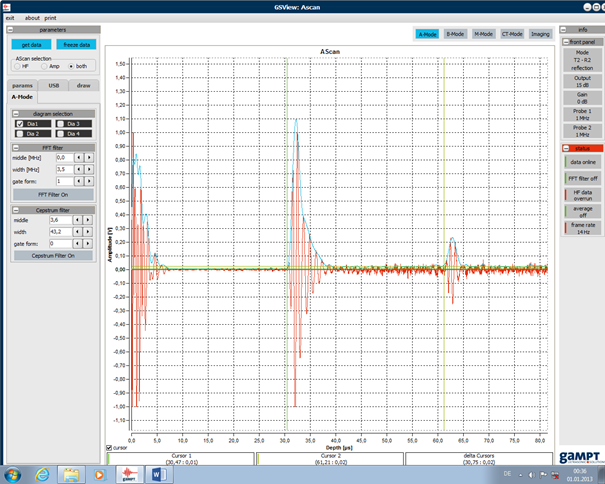
\includegraphics[width=\columnwidth]{img/Bild1.png}
\end{center}
\caption[]{Measuring runtimes in A-scan reflection mode. There are three peaks visible, the first one is the transmitted signal, the second one the received signal after being reflected once and the third peak is the received signal after being reflected twice. The cursors are placed at the start of the rising edge of the received signals to measure the time between sending and receiving the signals. The runtime of the second pulse is just twice that of the first.}
\label{fig:runtime}
\end{figure}

\section{Measuring the speed of sound}
The speed of sound $v_\text s$ in a material is important if any scale information is relevant, as the runtimes measured with the echoscope correspond to different travellenghts for different materials.

\subsection{Speed of sound in polyacryl, PVC and water}\label{sec:velo1}
As the echoscope allows us to measure the runtime $\tau$ of reflected sound pulses, these can be converted into the depth $d$ of a reflecting defect or material boundary by
\begin{align}\label{eq:dvt}
d=\frac{1}{2\,n}\,v_\text s\,\tau_\text n
\end{align}
where $n$ is the index of the peak and $v_\text s$ is the speed of sound in the material. Solving eq.~\ref{eq:dvt} for $v_\text s$, we can determine the speed of sound by measuring the actual distance with a caliper and determining the runtime of a signal pulse with the echoscope.\\\\
This was done for test cylinders of different lengths made of polyacryl and PVC with different sound frequencies to test for nonlinear dispersion as well as for a volume of water with a reflector placed in different distances to the transmitter. The results are given in Tab.~\ref{tab:velo1}.
\begin{table}[htbp]          %so funktionieren die Tabellen in LaTeX
\centering
\begin{tabular*}{\linewidth}{@{\extracolsep{\fill}}ccc}
\hline
\hline
\rule[-7pt]{0pt}{23pt}  Medium & Frequency [$\si\MHz$]  &  Speed of sound [$\frac{\si km}{\si s}$] 	 \\
\hline
\rule[-5pt]{0pt}{23pt}   polyacryl & $1$   &   $2,7144\pm0,0095$  	 \\
\rule[-5pt]{0pt}{23pt}   polyacryl & $2$   &   $2,7243\pm0,0086$  	 \\
\rule[-5pt]{0pt}{23pt}   PVC & $1$   &   $2,355\pm0,022$  	 \\
\rule[-5pt]{0pt}{23pt}   PVC & $2$   &   $2,3372\pm0,0012$  	 \\
\rule[-5pt]{0pt}{23pt}   water & $2$   &   $1,4864\pm0,0034$  	 \\
\hline
\hline
\end{tabular*}  
\normalsize
\caption[]{Sound velocities of polyacryl, PVC and water at different ultrasound frequencies.}  %siehe Graphik: Beschriftung
\label{tab:velo1}                             %siehe Graphik: zum Zitieren
\end{table}
For polyacryl and PVC, the two values at different frequencies coincide within the margin of error, so we could not observe a nonlinear dispersion relation for $1$ and $2\,\si\MHz$. The value for water coincides with the literature value  of $v_\text{water, theo}=1485\frac{\si\m}{\si\s}$ within the margin of error \cite{gerth}. For polyacryl and PVC there are no general literature values, as there are different chemical compositions of these materials.


\subsection{Speed of sound in copper and aluminum}
\begin{figure}[htbp]
\begin{center}
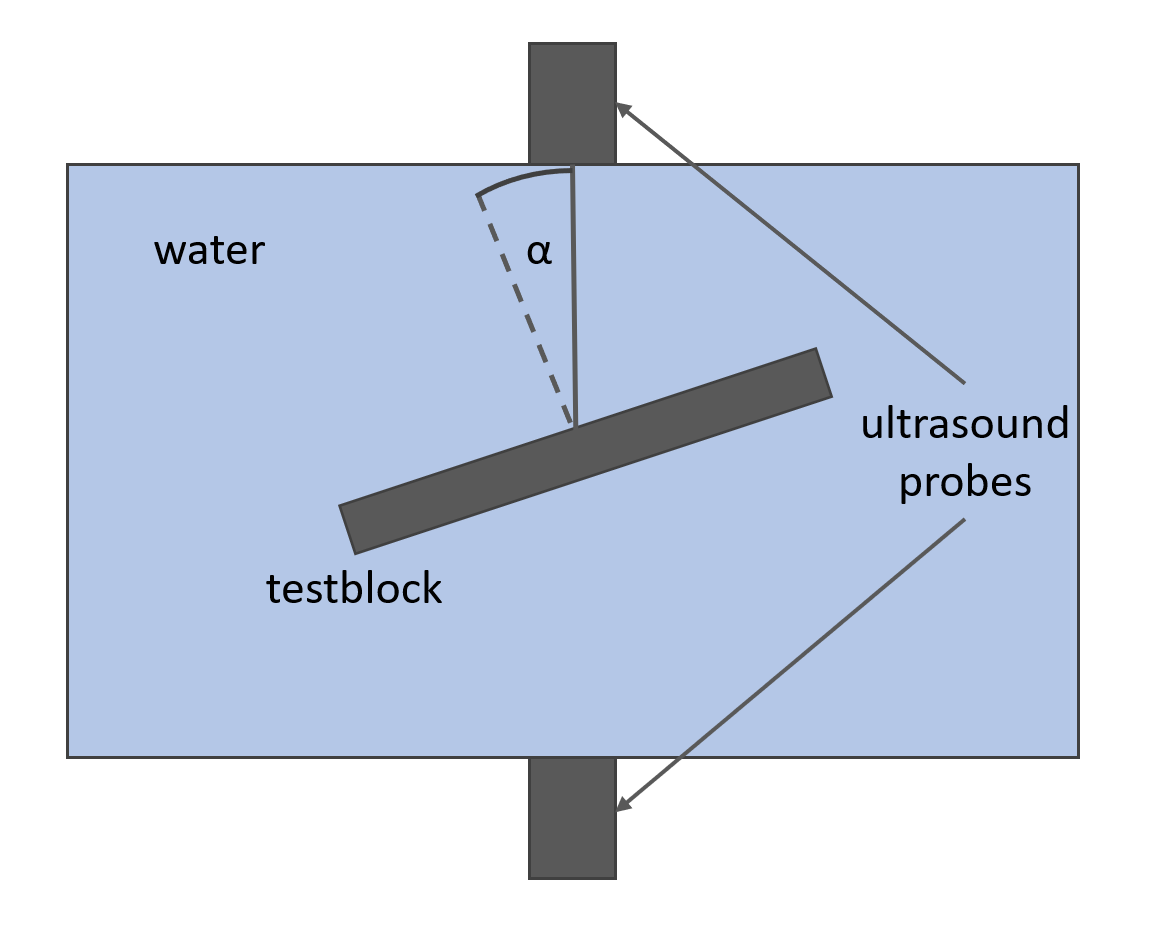
\includegraphics[width=\columnwidth]{img/C35-copper-alu-setup.png}
\end{center}
\caption[]{Schematic setup of the sound velocity measurement in copper and aluminum. A testblock is placed at different angles between two ultrasound probes measuring in transmission mode, with water in between as coupling.}
\label{fig:co-al-setup}
\end{figure}
Copper and aluminum are crystals with a specific periodic order of atoms. As the strength of their bounds depends on the direction, there are different sound velocities for different oscillation modes and we need a more sophisticated way of measuring them.\\
For this, we use the setup shown in Fig.~\ref{fig:co-al-setup}, where we place a block of the material we are testing in a water bath at different angles and the amplitudes of an A-scan are measured in transmission mode. At the boundary of the materials, we know that the angles of the incoming ($\alpha$) and refracted wave ($\beta$) follow Snell's law
\begin{align}
\frac{\sin \beta}{\sin \alpha}=\frac{v_\text{s}}{v_\text w}
\end{align}
\cite{instr} where $v_\text{w}$ is the speed of sound in water we already know from section~\ref{sec:velo1} and $v_\text{s}$ is the speed of sound in the solid. Performing an A-scan we should now get three peaks, one for each mode, where the peak with shortest runtime is that from the longitudinal mode and the two with longer runtimes are the transverse modes (see appendix section~\ref{sec:math}). We also know, that if $\beta = 90\si\degree$ there is total reflection for both longitudinal and transverse wave modes, so at the angle where the received signal of the corresponding mode vanishes, we can approximate $\beta = 90\si\degree$ and thus calculate $v_\text{s}$. On the other hand, transmission becomes maximal if $\beta = 45\si\degree$ for transverse waves \cite{instr}, so following the same logic we can get another value for the transverse mode at the maximum of the transverse peak. The measured intensities for the peaks of copper and aluminum are plotted in dependance of the angle $\alpha$ and shown in Fig.~\ref{fig:co} and \ref{fig:al}, where for copper we could only identify two peaks against the noise. We read off the highlighted angles with an estimated error of $2\si\degree$ for copper and $4\si\degree$ for aluminium to calculate the speeds of sound, which are given in Tab.~\ref{tab:velo2}.
\begin{figure}[htbp]
\begin{center}
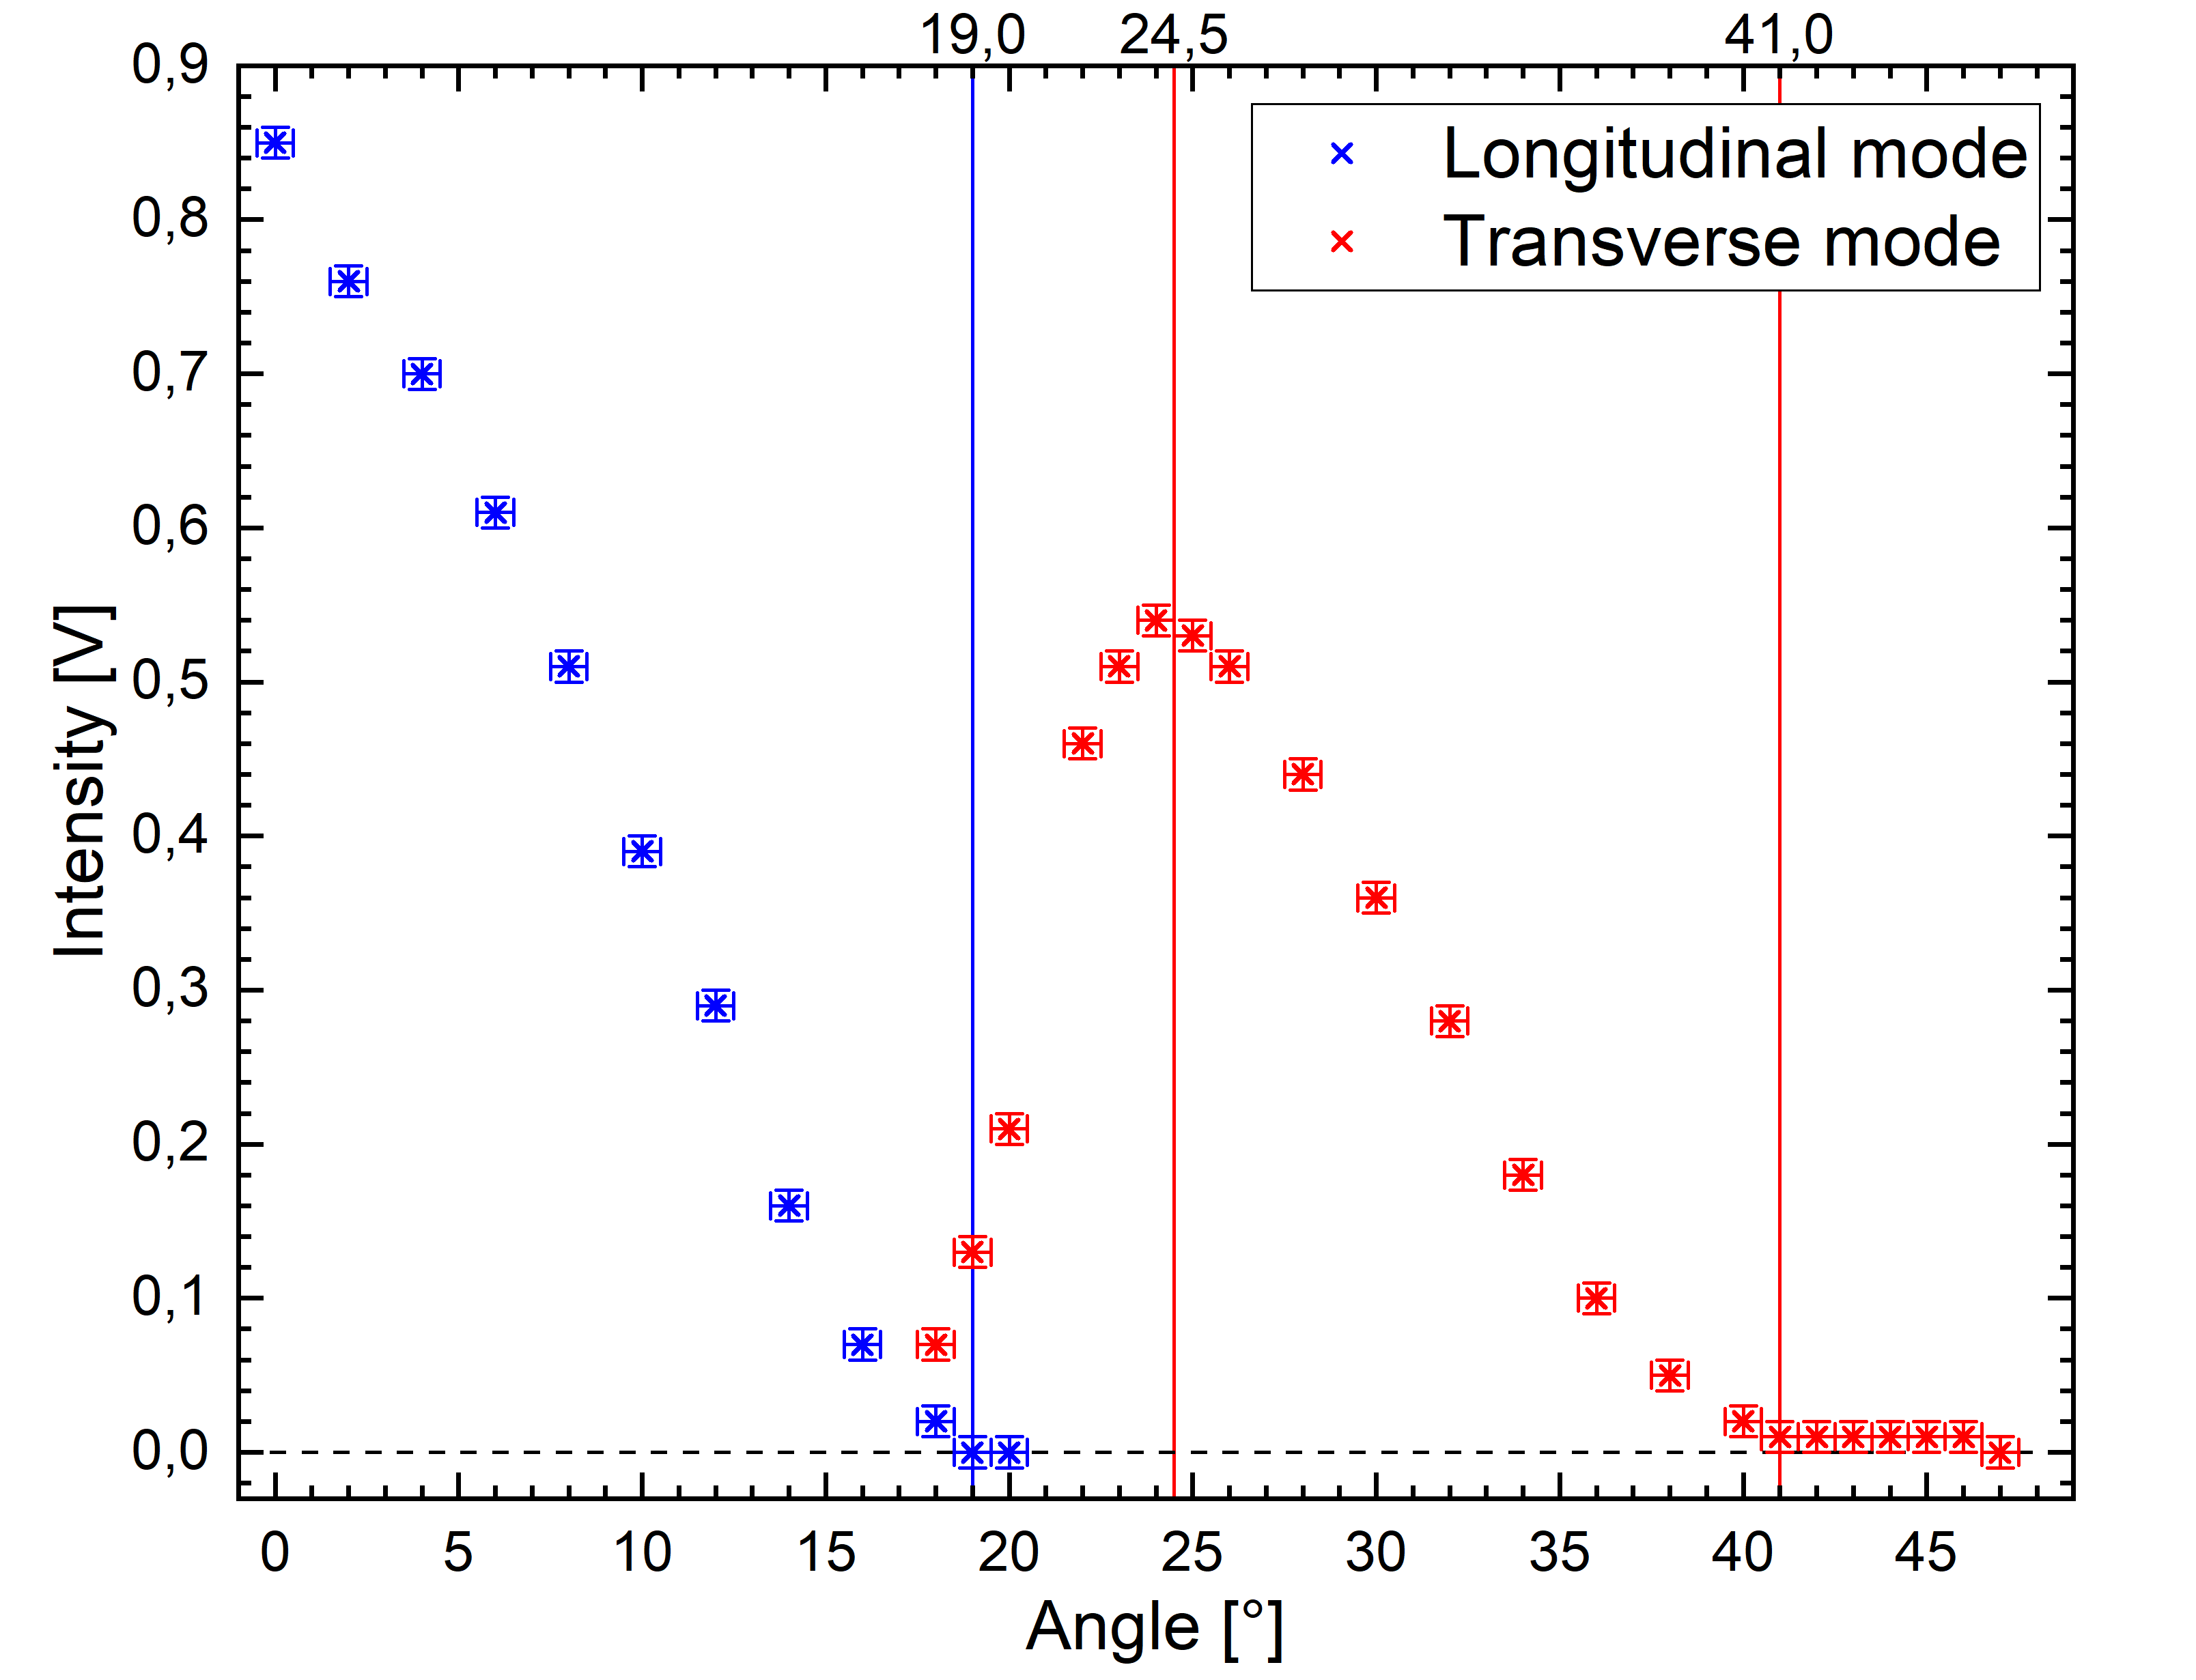
\includegraphics[width=\columnwidth]{img/SchallgeschwKupfer.png}
\end{center}
\caption[]{Intensity of transmitted ultrasound waves through a copper block at different angles. From the angles of maximum and minimum intensity the speeds of sound can be calculated for different modes.}
\label{fig:co}
\end{figure}
\begin{figure}[htbp]
\begin{center}
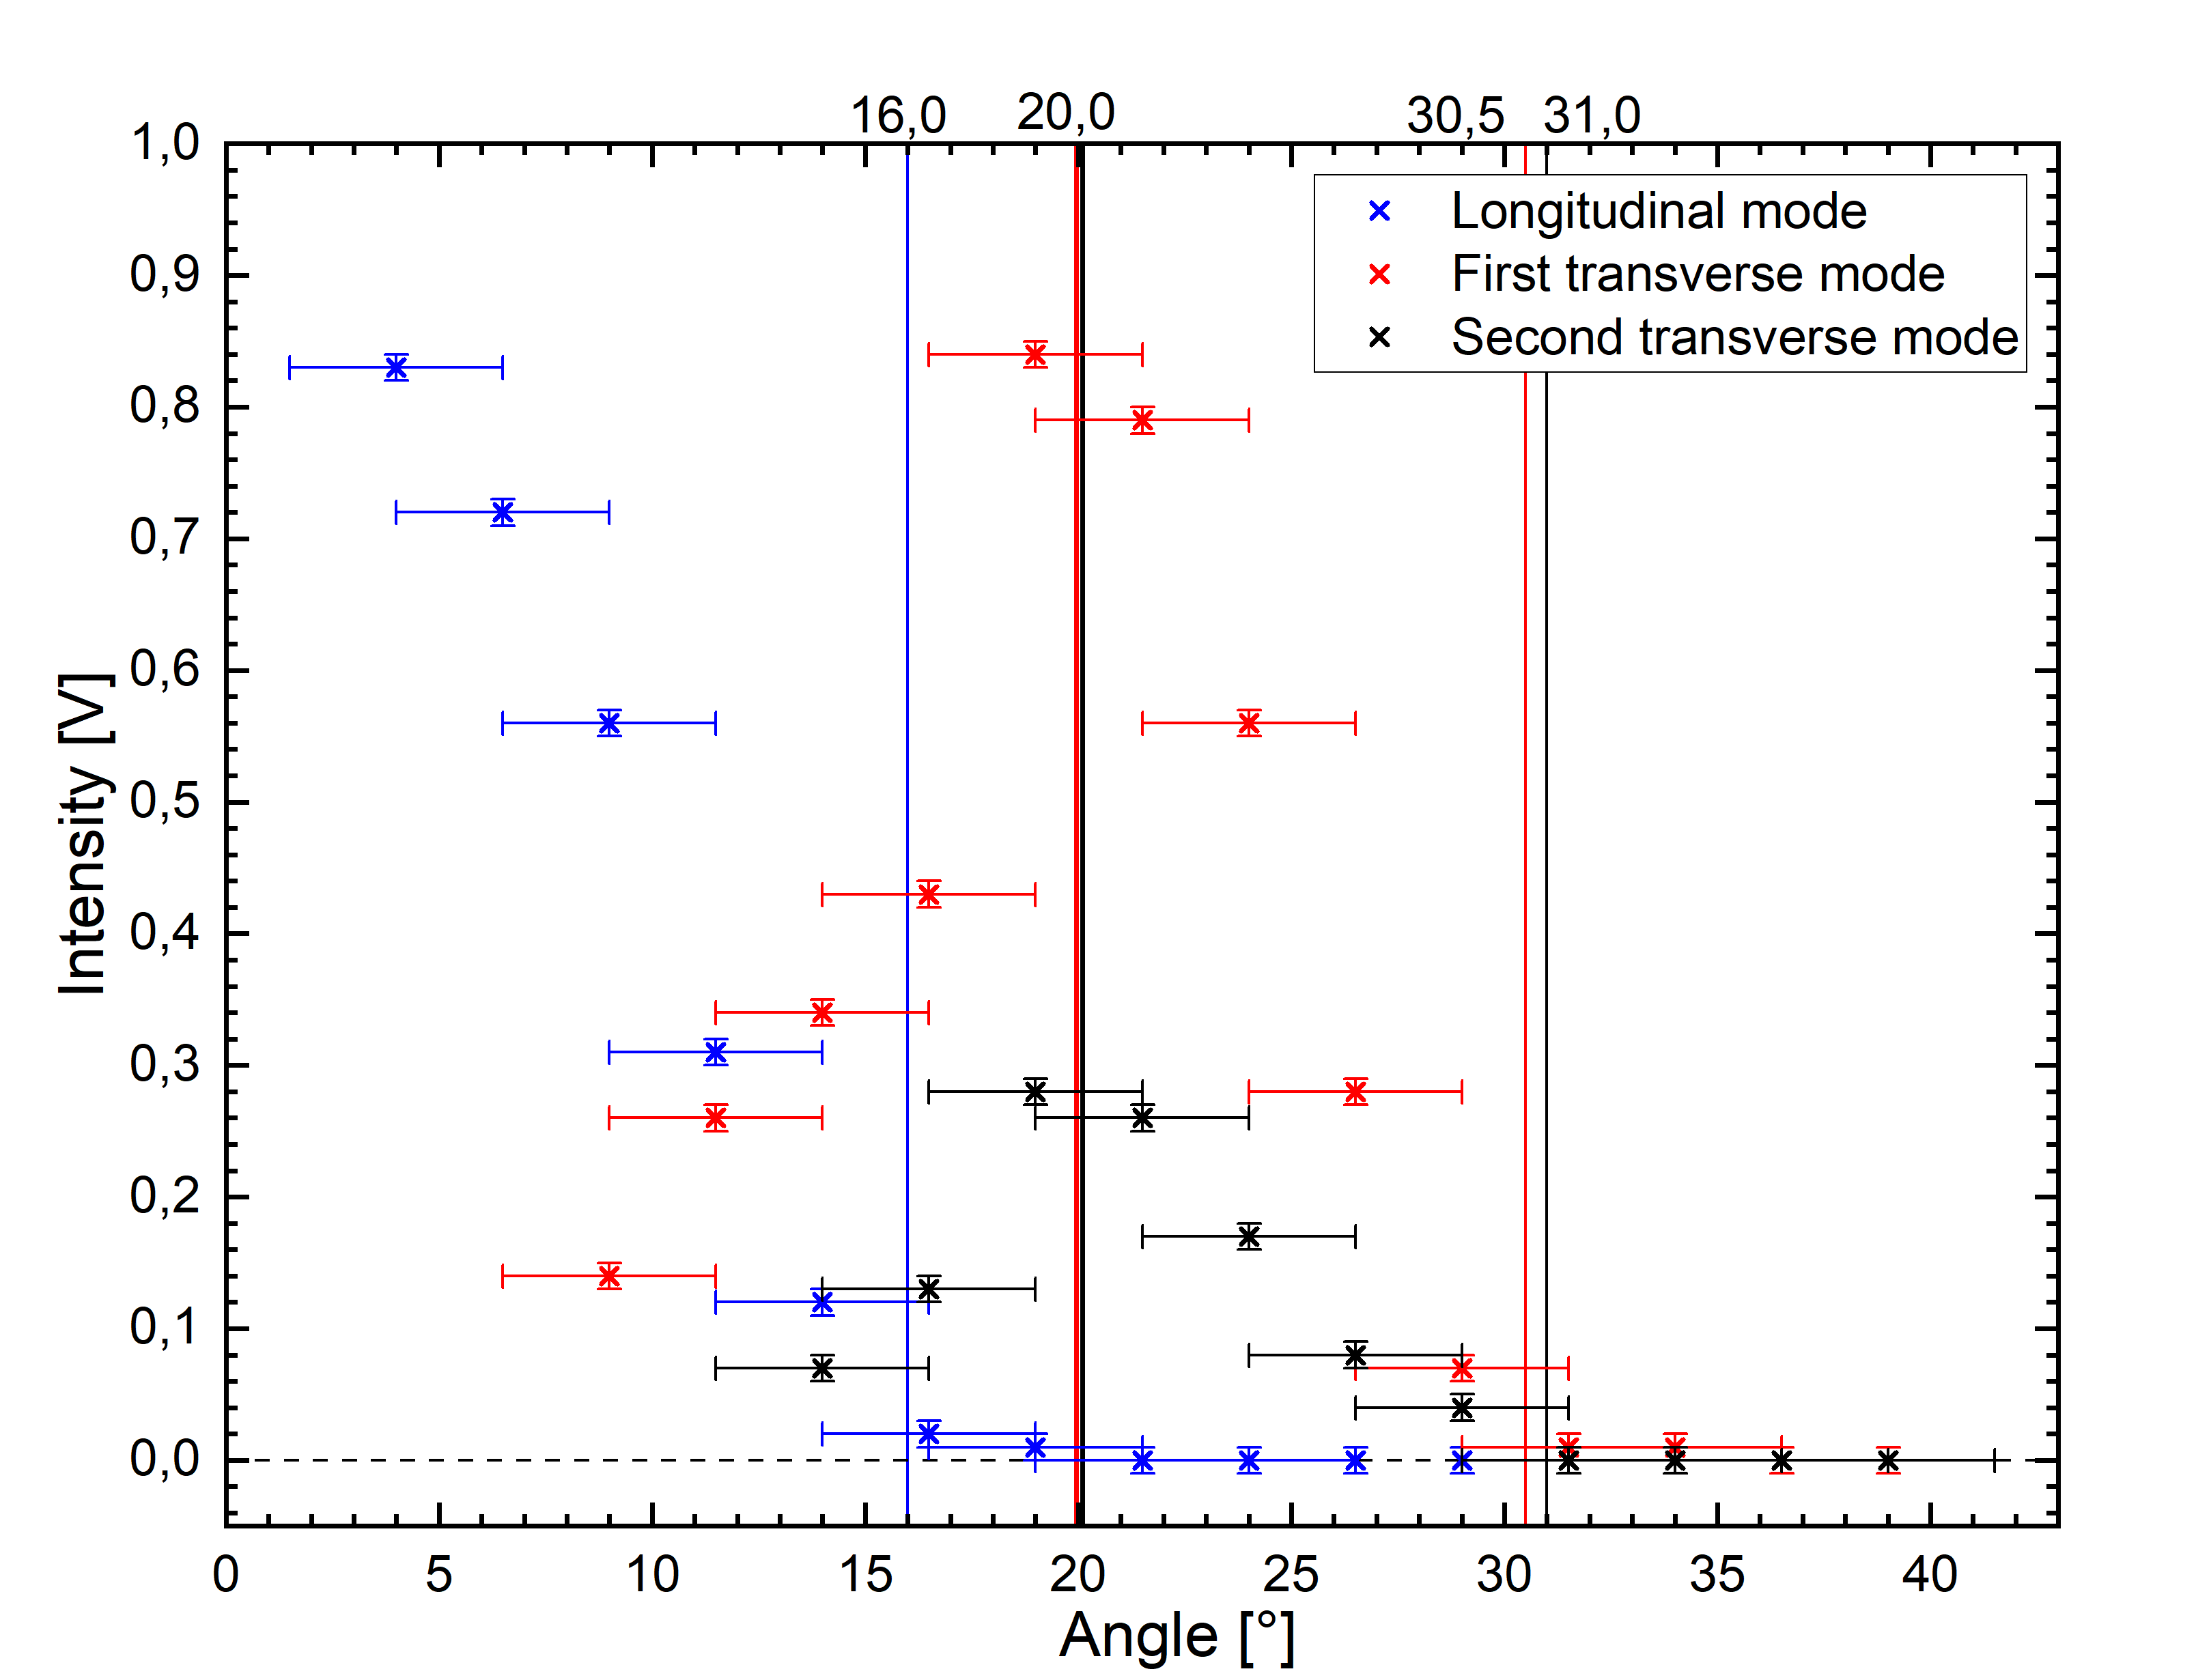
\includegraphics[width=\columnwidth]{img/SchallgeschwAlu.png}
\end{center}
\caption[]{Intensity of transmitted ultrasound waves through an aluminum block at different angles. From the angles of maximum and minimum intensity the speeds of sound can be calculated for different modes.}
\label{fig:al}
\end{figure}

\begin{table}[htbp]          %so funktionieren die Tabellen in LaTeX
\centering
\begin{tabular*}{\linewidth}{@{\extracolsep{\fill}}cccc}
\hline
\hline
\rule[-7pt]{0pt}{23pt}  Medium & Mode  & $\beta$ [$\si\degree$] &  $v$ [$\frac{\si km}{\si s}$] 	 \\
\hline
\rule[-5pt]{0pt}{23pt}   copper & longitudinal  &   $90$ &   $4,57\pm0,46$  	 \\
\rule[-5pt]{0pt}{23pt}   copper & transverse  &   $45$ &   $2,53\pm0,19$  	 \\
\rule[-5pt]{0pt}{23pt}   copper & transverse &   $90$  &   $2,266\pm0,091$  	 \\
\rule[-5pt]{0pt}{23pt}   aluminium & longitudinal  &   $90$ &   $5,4\pm1,3$  	 \\
\rule[-5pt]{0pt}{23pt}   aluminium & first transverse  &   $45$ &   $3,07\pm0,59$  	 \\
\rule[-5pt]{0pt}{23pt}   aluminium & first transverse  &   $90$ &   $2,93\pm0,35$  	 \\
\rule[-5pt]{0pt}{23pt}   aluminium & second transverse  &   $45$ &   $3,07\pm0,59$  	 \\
\rule[-5pt]{0pt}{23pt}   aluminium & second transverse &   $90$  &   $2,89\pm0,34$  	 \\
\hline
\hline
\end{tabular*}  
\normalsize
\caption[]{Sound velocities $v$ in copper and aluminum for different wave modes for ultrasound of the frequency $f=2\,\si\MHz$.} %siehe Graphik: Beschriftung
\label{tab:velo2}                             %siehe Graphik: zum Zitieren
\end{table}

Our measurement follows the theory, as the values for both the longitudinal and transverse modes in copper and aluminum lie within the expected ranges of the theoretical calculations (see appendix, Tab.~\ref{tab:theoVelo}) within the margins of error, even though we cannot quantitatively confirm the shape of the theoretical curves (see appendix, Fig.~\ref{fig:al-theo} and \ref{fig:co-theo}) as there is no information on the orientation of the crystals.
 

\section{Absorption of ultrasound in PVC}\label{sec:abs}
In all our experiments, the ultrasound waves were damped when travelling through the medium, which we had to compensate by amplifying our signal using overall gain as well as time gain control (TGC), a function of the echoscope that allows us to increase amplification with runtime, so pulses with long runtimes would be visible while the others would not be overdriven.\\\\
We now want to quantify the absorption of the waves in PVC. For damped waves we expect the intensity $I$ to decrease exponentially with distance $x$ following
\begin{align}
I(x)\sim e^{-\lambda x}
\end{align}
with an absorption coefficient $\lambda$. To determine this coefficient, we first switched off TGC, set a fixed input amplification (gain) and measured the amplitudes of the signal for different lengths of PVC cylinders. Fitting an exponential function to the data, we obtained $\lambda_\text{1MHz} = (0,2752\pm0,0093)\,\si\cm^{-1}$ and $\lambda_\text{2MHz} = (0,459\pm0,057)\,\si\cm^{-1}$.\\
The absorption is stronger for higher frequencies due to the faster oscillation of the atoms. This leads to a faster scattering process of the ordered wave resulting in unordered oscillations, thus an energy loss in form of heat is observed.

\section{Resolution of ultrasound imaging}\label{sec:res}
The wave pulses sent by the echoscope are of finite length rather than $\delta$-functions. For that reason, it is not possible to separate reflection sources that are too close to each other, as then the pulses overlap and can not be distinguished anymore. To quantify the resolution of an ultrasound measurement, we choose the full width at half maximum (FWHM) of the peaks, as it is invariant under amplification. We say that two peaks are distinguishable, if their distance is at least the FWHM. This quantity was measured for different sound frequencies at the same defect (bore $3$ of the polyacryl testblock from Fig.~\ref{fig:testblock}) and the values are given in Tab.~\ref{tab:res}.
\begin{table}[htbp]          %so funktionieren die Tabellen in LaTeX
\centering
\begin{tabular*}{\linewidth}{@{\extracolsep{\fill}}cc}
\hline
\hline
\rule[-7pt]{0pt}{23pt}  Frequency [$\si\MHz$] &  FWHM [$\si{\micro\s}$] 	 \\
\hline
\rule[-5pt]{0pt}{23pt}   $1$ &    $1,70\pm0,01$  	 \\
\rule[-5pt]{0pt}{23pt}   $2$ &    $1,18\pm0,01$  	 \\
\rule[-5pt]{0pt}{23pt}   $4$ &    $0,69\pm0,01$  	 \\
\hline
\hline
\end{tabular*}  
\normalsize
\caption[]{Full width half maximum (FHWM) of ultrasound pulses at different frequencies as an indicator for resolution. Clearly, a higher frequency provides a better resolution. The values were all measured after reflection of the signal at the third bore of the polyacryl testblock.} %siehe Graphik: Beschriftung
\label{tab:res}                             %siehe Graphik: zum Zitieren
\end{table}
\\\\Analogous to optics, our data shows that a higher frequency and thus a smaller wavelength provides a better resolution. This means, that choosing a higher frequency should result in a more accurate measurement, but with the result of section~\ref{sec:abs} we also know that higher frequencies are absorbed faster, which leads to a less accurate measurement. So ultimately for the frequency a compromise between resolution and absorption needs to be made, which is why we used the $2\,\si\MHz$ probe most of the time.

\section{Non destructive material analysis with ultrasound imaging}
Ultrasound allows us to gain information about the inside of a material without destroying it to actually look inside. To understand the basics of this technique, we use a testblock of polyacryl with eleven bores that go all the way through the block, schematically depicted in Fig.~\ref{fig:testblock}.

\begin{figure}[htbp]
\begin{center}
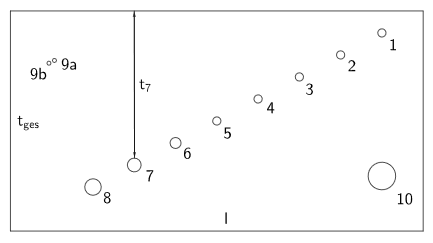
\includegraphics[width=\columnwidth]{img/testblock.png}
\end{center}
\caption[]{Schematic picture of the polyacryl testblock. The runtimes $t_\text i$ from the top of the block to the different bores were measured and converted into lengths via the speed of sound in polyacryl \cite{echoscope}.}
\label{fig:testblock}
\end{figure}

\subsection{B-picture}
We performed a B-scan of the testblock from Fig.~\ref{fig:testblock} as described in section~\ref{sec:echoscope}. The result can be seen in Fig.~\ref{fig:B-scan}.
\begin{figure}[htbp]
\begin{center}
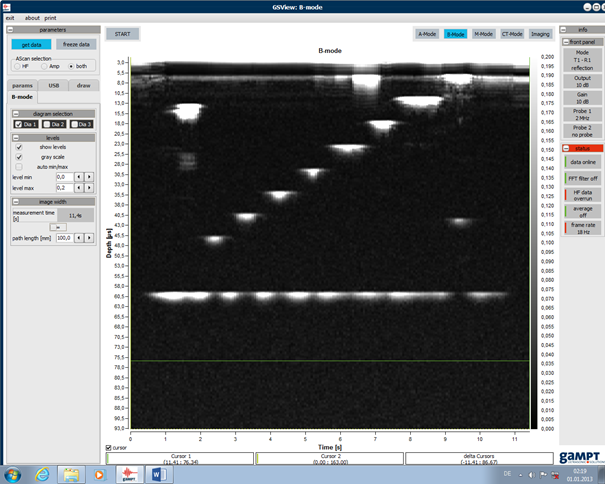
\includegraphics[width=\columnwidth]{img/Bild18.png}
\end{center}
\caption[]{$2D$ B-picture of a testblock. The bright spots are bores reflecting the signal. The different lengths of the bright spots in horizontal direction have no physical meaning, as the echoscope plots the time after start of the measurement on that axis and the probe just could not be moved with a perfectly constant velocity, so local stretching appears.}
\label{fig:B-scan}
\end{figure}
The bright spots in the scan indicate structural changes in the the material where ultrasound waves were reflected. In our case these are bores in the testblock, but in industrial applications they can be material defects or filling levels of liquids while in medicine B-scans are used to identify different structures inside a living body.

\subsection{Length measurements}
As we know the speed of sound in polyacryl from section~\ref{sec:velo1}, we can calculate the depths $d_\text i$ of the bores from runtime measurements in reflective A-scan mode. These were performed with the $f=2\,\si\MHz$ probe. For reference, the same depths were measured with a caliper and the results are given in Tab.~\ref{tab:testblock}. We also tried to measure the distance between bores $9a$ and $9b$ with different frequencies of the waves to further confirm our observation on the resolution from section~\ref{sec:res}. As this distance is too small we could not measure the start of the rising edge as described in section~\ref{sec:runtime} and had to use a peak to peak measurement. For the same reason the start of the rising edge of the $9b$ peak had to be approximated to measure $d_\text{9b}$.
\begin{table}[htbp]          %so funktionieren die Tabellen in LaTeX
\centering
\begin{tabular*}{\linewidth}{@{\extracolsep{\fill}}ccc}
\hline
\hline
\rule[-7pt]{0pt}{23pt}  Bore & $d_\text{caliper}\,[\si\mm]$ & $d_\text{ultrasound}\,[\si\mm]$ 	 \\
\hline
\rule[-15pt]{0pt}{23pt}   $d_\text{tot}$ & $80,21\pm0,03$  &  $80,12\pm0,25$  	 \\
\rule[-15pt]{0pt}{23pt}   $d_\text 1$ &   $6,90\pm0,03$ &  $7,001\pm0,026$  	 \\
\rule[-15pt]{0pt}{23pt}   $d_\text 2$ &  $14,95\pm0,03$ &  $14,970\pm0,049$  	 \\
\rule[-15pt]{0pt}{23pt}   $d_\text 3$ &  $22,93\pm0,03$ &  $22,952\pm0,074$  	 \\
\rule[-15pt]{0pt}{23pt}   $d_\text 4$ &  $30,93\pm0,03$ &  $30,907\pm0,098$  	 \\
\rule[-15pt]{0pt}{23pt}   $d_\text 5$ &  $38,87\pm0,03$ &  $38,86\pm0,12$  	 \\
\rule[-15pt]{0pt}{23pt}   $d_\text 6$ &  $46,67\pm0,03$ &  $46,59\pm0,15$  	 \\
\rule[-15pt]{0pt}{23pt}   $d_\text 7$ & $53,94\pm0,03$ &   $53,87\pm0,17$  	 \\
\rule[-15pt]{0pt}{23pt}   $d_\text 8$ &  $61,41\pm0,03$ &  $61,38\pm0,19$  	 \\
\rule[-15pt]{0pt}{23pt}   $d_\text{9a}$ &  $17,46\pm0,03$ &  $17,545\pm0,057$  	 \\
\rule[-15pt]{0pt}{23pt}   $d_\text{9b}$ &  $19,12\pm0,03$ &  $19,588\pm0,063$  	 \\
\rule[-15pt]{0pt}{23pt}   $d_\text{10}$ &  $55,41\pm0,03$ &  $55,36\pm0,18$  	 \\
\rule[-15pt]{0pt}{23pt}   $\Delta d_\text 9(f=1\,\si\MHz)$ &    $1,66\pm0,04$& $1,907\pm0,015$   	 \\
\rule[-15pt]{0pt}{23pt}   $\Delta d_\text 9(f=2\,\si\MHz)$ & $1,66\pm0,04$ &    $1,662\pm0,015$  	 \\
\rule[-15pt]{0pt}{23pt}   $\Delta d_\text 9(f=4\,\si\MHz)$ &$1,66\pm0,04$ &    $1,703\pm0,015$  	 \\
\hline
\hline
\end{tabular*}  
\normalsize
\caption[]{Length measurements on a testblock with a caliper and ultrasound} %siehe Graphik: Beschriftung
\label{tab:testblock}                             %siehe Graphik: zum Zitieren
\end{table}
\\\\The measurement with ultrasound coincides with the caliper measurement within the margin of error in $80\%$ of the measured cases. $d_\text{9b}$ and $\Delta d_\text 9(f=1\,\si\MHz)$ not coinciding can be explained with the result from section~\ref{sec:res}, as bores $9a$ and $9b$ are too close to separate the two peaks. Excluding those two cases, the correspondance is $92\%$. This shows, that length measurements with ultrasound are very accurate, as long as the frequency is high enough to resolve all important details and the medium is isotropic such that the speed of sound is the same everywhere.


\section{Conclusion}
In this experiment, we first determined the speed of ultrasound in different materials at an ultrasound frequency of $f=2\,\si\MHz$. For the isotropic materials polyacryl, PVC and water we received $v_\text{polyacryl}= (2,7243\pm0,0086) \,\frac{\si\km}{\si\s}$, $v_\text{PVC}= (2,3372\pm0,0012) \,\frac{\si\km}{\si\s}$ and $v_\text{water}= (1,4864\pm0,0034) \,\frac{\si\km}{\si\s}$ which coincide with the literature values within the margin of error. For polyacryl and PVC we also performed the same measurement with $f=1\,\si\MHz$, but could not identify a nonlinear dispersion within the margin of error. We also measured the speed of sound in copper and aluminum, each for the longitudinal and the transverse modes. For the longitunial modes we received $v_\text{l, co}= (4,57\pm0,46)\,\frac{\si\km}{\si\s}$ and $v_\text{l, al}= (5,4\pm1,3)\,\frac{\si\km}{\si\s}$, while the transverse velocities are in the ranges $v_\text{t, co}\in [(2,53\pm0,19)\,\frac{\si\km}{\si\s}, (2,266\pm0,091)\,\frac{\si\km}{\si\s}]$ and $v_\text{t, al}\in [(2,89\pm0,34)\,\frac{\si\km}{\si\s}, (3,07\pm0,59)\,\frac{\si\km}{\si\s}]$. These values also coincide with the theoretical expectation. We then measured the absorption coefficients for the intensity of ultrasound in PVC for two frequencies to be $\lambda_\text{1MHz} = (0,2752\pm0,0093)\,\si\cm^{-1}$ and $\lambda_\text{2MHz} = (0,459\pm0,057)\,\si\cm^{-1}$, so higher frequencies are absorbed more strongly. Defining the full width at half maximum (FHWM) of an ultrasound pulse as an indicator for the resolution, we found that the resolution of ultrasound imaging increases with frequency, while a $4\,\si\MHz$ signal has a $59\%$ smaller FWHM than a  $1\,\si\MHz$ signal. At last, we performed some non destructive material analysis by taking a B-scan of a testblock and measuring distances in the same block with ultrasound as well as a caliper. $92\%$ of the values where the distance was not below the resolution of the soundwaves coincide within the margin of error. Measuring the smallest distance in the test block we could see again that this was only possible for the higher ultrasound frequencies, confirming our observation on the resolution.

\FloatBarrier

%FF: Angabe der verwendeten Literatur mit Quellennachweis.
\begin{thebibliography}{}    %so wird das Literaturverzeichnis erstellt
\bibitem{instr} Physikalisches Grundpraktikum, Universit�t W�rzburg, Modul C2, Versuch 35, \grqq Messungen mit Ultraschall\grqq, 2021 
\bibitem{gerth} Meschede, Dieter, Gerthsen Physik, 25. Auflage, Springer-Verlag, Berlin, 2015 
\bibitem{codata} E. Tiesinga \textit{et al.}, \grqq CODATA
recommended values of the fundamental physical constants: 2018\grqq, Rev. Mod. Phys. 93, 025010 (2021)
\bibitem{echoscope} Gampt mbH, \grqq ULTRASCHALLECHOSKOP 
GS200/GS200i\grqq, Version 0.70 DE, 08. Dezember 2015

\end{thebibliography}


\newpage\,
\section{Appendix}
\subsection{Mathematical description of wave propagation in a crystal}\label{sec:math}
Mechanical waves are described by a set of differential equations
\begin{align}
\rho\frac{\partial^2u_\text i}{\partial t^2}=\sum_\text{jkl} c_\text{ijkl} \frac{\partial^2u_\text l}{\partial x_\text j \partial x_\text k}
\end{align}
where $u_\text i$ is the displacement in $x_\text i$-direction and $c$ is the Young's modulus. Solving these equations for the case that the waves travel in the $x-y$ plane, we receive the theoretical, angular dependent speed of sound for a longitudinal and two transverse modes. Fig.~\ref{fig:al-theo} and \ref{fig:co-theo} show angular plots of these velocities. Here it becomes clear, that the longitudinal velocity is always larger than the transverse velocities, thus pulses in the longitudinal mode have the shortest runtime. For copper, depending on the angle the two transverse modes can be differentiated quite well, while in aluminum their velocities are very similar.  The theoretical values for longitudinal  and extremal transverse speed of sound are given in Tab.~\ref{tab:theoVelo}.
\begin{figure}[htbp]
\begin{center}
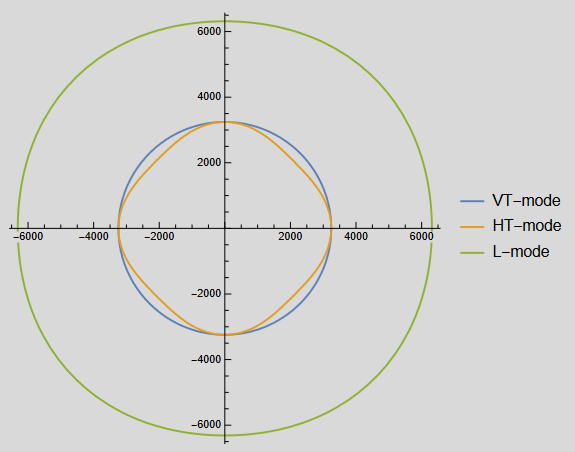
\includegraphics[width=\columnwidth]{img/co-theo.png}
\end{center}
\caption[]{Theoretical speed of sound in $\frac{\si\m}{\si\s}$ in aluminum for different wave modes in dependence of the orientation inside the crystal. L-mode is the longitudinal mode, HT the transverse mode in the plane of propagation and VT the transverse mode perpendicular to the plane of propagation.}
\label{fig:al-theo}
\end{figure}
\begin{figure}[htbp]
\begin{center}
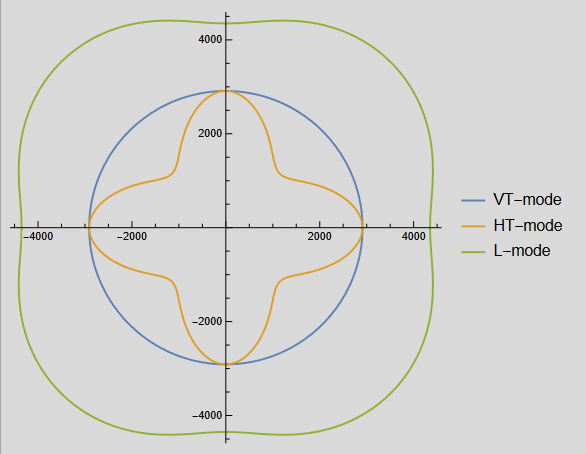
\includegraphics[width=\columnwidth]{img/al-theo.png}
\end{center}
\caption[]{Theoretical speed of sound in $\frac{\si\m}{\si\s}$ in copper for different wave modes in dependence of the orientation inside the crystal. L-mode is the longitudinal mode, HT the transverse mode in the plane of propagation and VT the transverse mode perpendicular to the plane of propagation.}
\label{fig:co-theo}
\end{figure}

\begin{table}[htbp]          %so funktionieren die Tabellen in LaTeX
\centering
\begin{tabular*}{\linewidth}{@{\extracolsep{\fill}}cccc}
\hline
\hline
\rule[-7pt]{0pt}{23pt}  Medium & Mode &  $c_\text{s,max}$[$\frac{\si km}{\si s}$] & $c_\text{s,min}$[$\frac{\si km}{\si s}$]	 \\
\hline
\rule[-5pt]{0pt}{23pt}   copper & longitudinal   &   $4,9755$ & $4,35011$  	 \\
\rule[-5pt]{0pt}{23pt}   copper & transverse   &   $2,91082$ & $1,62504$ 	 \\
\rule[-5pt]{0pt}{23pt}   aluminium & longitudinal  &   $6,46376$ & $6,31333$ 	 \\
\rule[-5pt]{0pt}{23pt}   aluminium & transverse   &   $3,24413$ & $2,93298$ 	 \\
\hline
\hline
\end{tabular*}  
\normalsize
\caption[]{Theoretical values for the sounds of speed in copper and aluminium, depending on the wave mode.}  %siehe Graphik: Beschriftung
\label{tab:theoVelo}                             %siehe Graphik: zum Zitieren
\end{table}


\end{document}
